% Chapter Template

\chapter{Agile and Correct by Construction} % Main chapter title

\label{Chapter_Agile_and_Correct_by_Construction} % Change X to a consecutive number; for referencing this chapter elsewhere, use \ref{ChapterX}

%----------------------------------------------------------------------------------------


\section{Agile Software Development}

\subsection{Manifesto for Agile Software Development}

The manifesto sets out the overarching principles of agile software development \parencite{Beck2001ManifestoFA}:

\begin{displayquote}
We are uncovering better ways of developing software by doing it and helping 
others do it. Through this work we have come to value:

\begin{itemize}
	\item \textbf{Individuals and interactions} \textit{over} processes and tools 
	\item \textbf{Working software} \textit{over} comprehensive documentation 
	\item \textbf{Customer collaboration} \textit{over} contract negotiation 
	\item \textbf{Responding to change} \textit{over} following a plan 
\end{itemize}

That is, while there is value in the items on the right, we value the items on
the left more.
\end{displayquote}

\subsection{Agile Software Development using Scrum}
Scrum is an agile project management methodology. It focuses on short feedback
loops all development process. The client is involved in all iterations of the process
ensuring that the completed project meets the client's needs and expectations \parencite{ScrumGoesFormal}.

\subsubsection{Scrum roles}
There are three roles in Scrum \parencite{ScrumGoesFormal}:
\begin{description}
	\item [Product Owner:] This person represents the customer’s interest, and 
		determines the goal of each iteration. It is the product owner's responsibility
		to prioritise the different tasks ensuring that the most important functionality
		is implemented first.
	\item [Scrum Master:] It is the Scrum Master's responsibility to facilitate the Scrum 
		process and protect the agile principles. He also needs to protect the team by
		removing any impediments encountered by the team, ensuring that the team is not
		distracted from the task at hand.
	\item [Team:] A team consists of five to nine people working together to create
		a functional system which satisfies the user needs. The team consists of people
		with a broad set of competences so that the team is self-organised and contained.
\end{description}

\subsubsection{Activities and Artifacts}
Scrum has several activities, that describe the development workflow, and artifacts,
that are produced by the process \parencite{ScrumGoesFormal}:
\begin{description}
	\item [Product vision:] This is the initial idea phase. The vision of the 
		product is defined during this process.
	\item [Product backlog:] This is a prioritised list of artifacts that are needed
		in the product. The artifacts are described as user stories, the story describes
		how we are adding value for the user.
	\item [Sprint:] This is the development iteration. Sprints are time boxed between
		 two to six weeks.
	\item [Sprint planning:] The first day of each sprint is used to plan what is
		going to be done during the sprint.
	\item [Sprint backlog:] These are the stories, from the product backlog the team
		has committed to implementing in the sprint.
	\item [Daily Scrum meeting:] This is a short, 15 minutes, daily meeting used to plan
		the days work and checking on the state of the stories in the sprint.
	\item [Sprint review:] The meeting is held at the end of the sprint to show the 
		product owner the work that has been completed during the sprint.
	\item [Sprint retrospective:] This meeting is held after the sprint review. The 
		focus of the meeting is not on the work completed during the. The purpose
		of the meeting is to discuss the people, relationships, processes, and tools 
		in order to improve the team's effectiveness.
\end{description}

\begin{figure}[H]
	\centering
	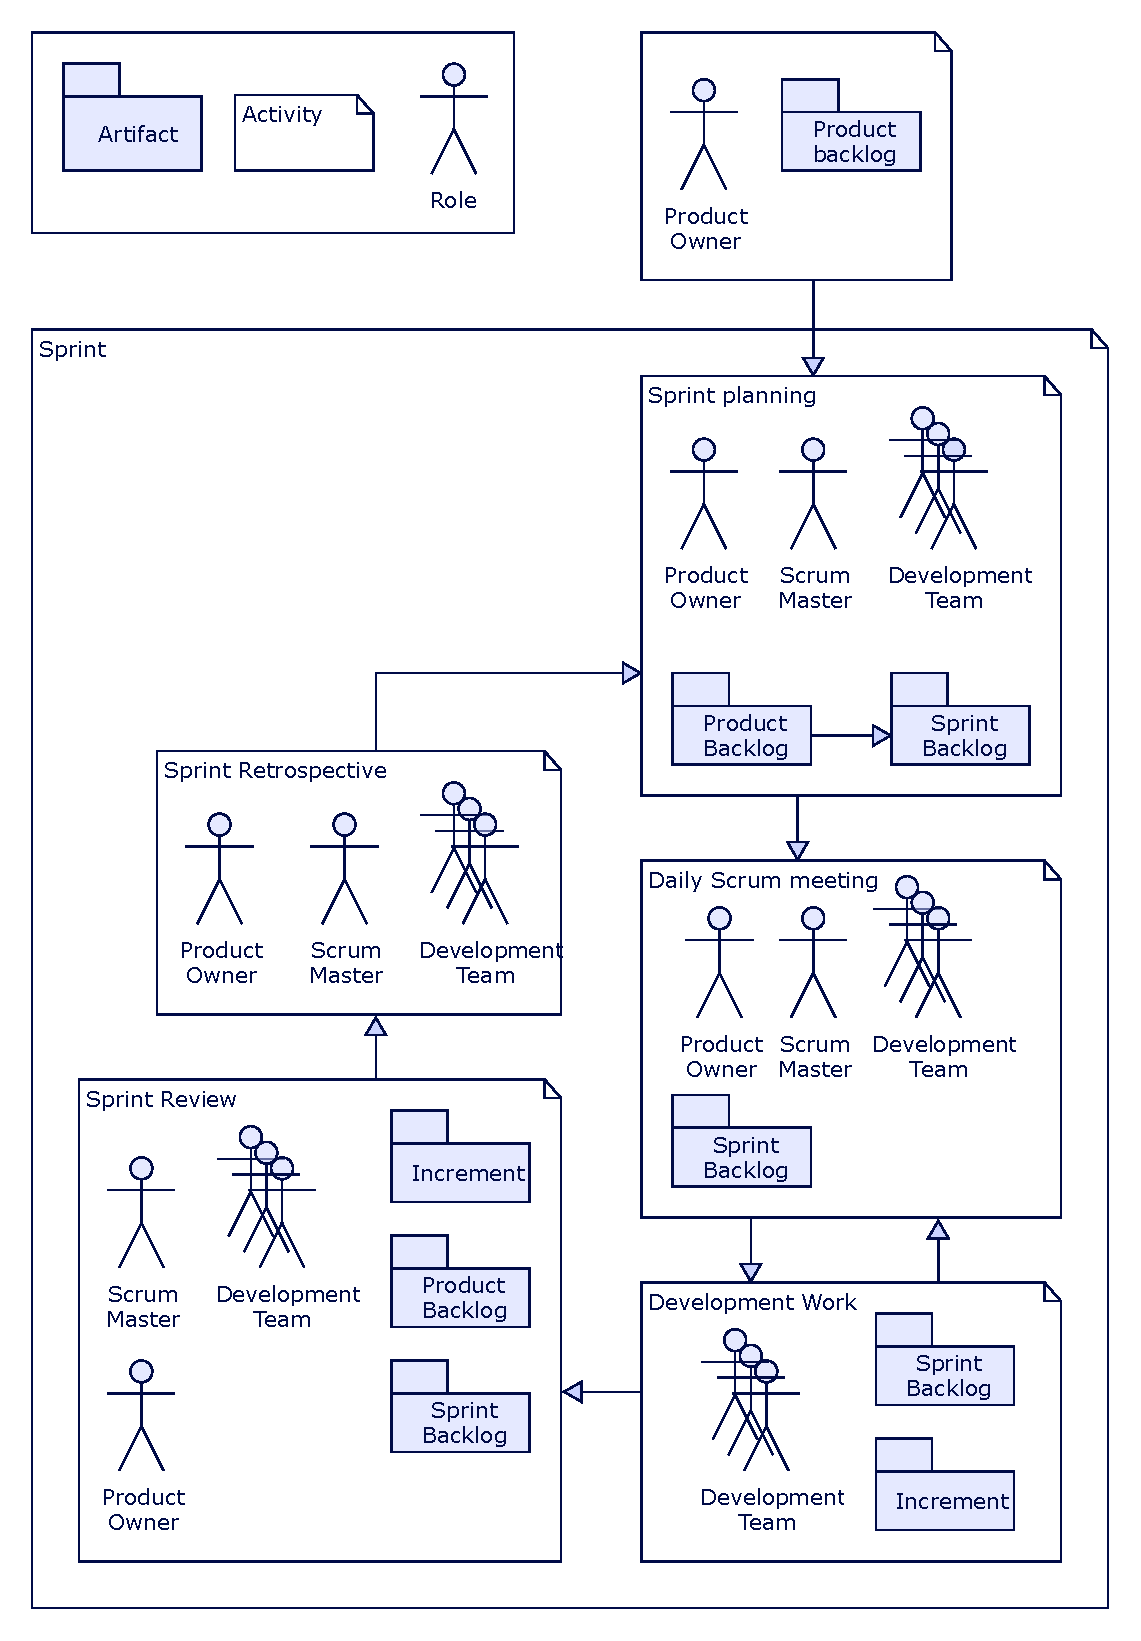
\includegraphics[scale=0.75]{Figures/Scrum_workflow.pdf}
	\decoRule
	\caption{The scrum workflow.}
	\label{fig:ScrumWorkflow}
\end{figure}

\section{Using CbyC in Agile Scrum}

The strived for characteristic of agile software development is the ability to 
react to change. With scrum we will have to implement the change in order to test
it. If we evaluate this against the Agile manifesto:
\begin{description}
	\item [Responding to change:]  In order to evaluate a change: a story has to be
		create, and the story has to be refined and sized. Then, depending on the 
		priority, existing work has to be moved to make resources available to implement
		the change. 
	\item [Working software:] We have to implement the requested change in order to
		validate it. If the change does not work we might end up with invalid or
		non-functional software.
	\item [Customer collaboration] For a change to be actioned the team will reason
		through it on a whiteboard. This reasoning is based on opinion and results in
		arguments that cannot be resolved without implementing the change.
\end{description}

If we now augment our agile scrum workflow with CbyC the process changes as shown in  Figure \ref{fig:ScrumCbyCWorkflow}.

\subsubsection{Roles}
\begin{description}
	\item [Team Architect:] This person helps the Product Owner to create the formal
		specification. This role can be shared amongst the team members and does not
		have to belong to a specific person.
\end{description}

\subsubsection{Activities and Artifacts}
\begin{description}
	\item [Product Vision:] Here the Team Architect incorporates the Product Owner's
		requirements into the Formal Specification. The Formal Specification is then 
		validated. If the requirements are valid stories are created on the Product
		Backlog.
	\item [Sprint:] During the sprint we now incorporate the Formal Design, System
		Test Specification, INFORMED Design, and Code Implementation in our development
		process as described in paragraph \ref{CbyCDevWorkflow}
\end{description}

\begin{figure}[H]
	\centering
	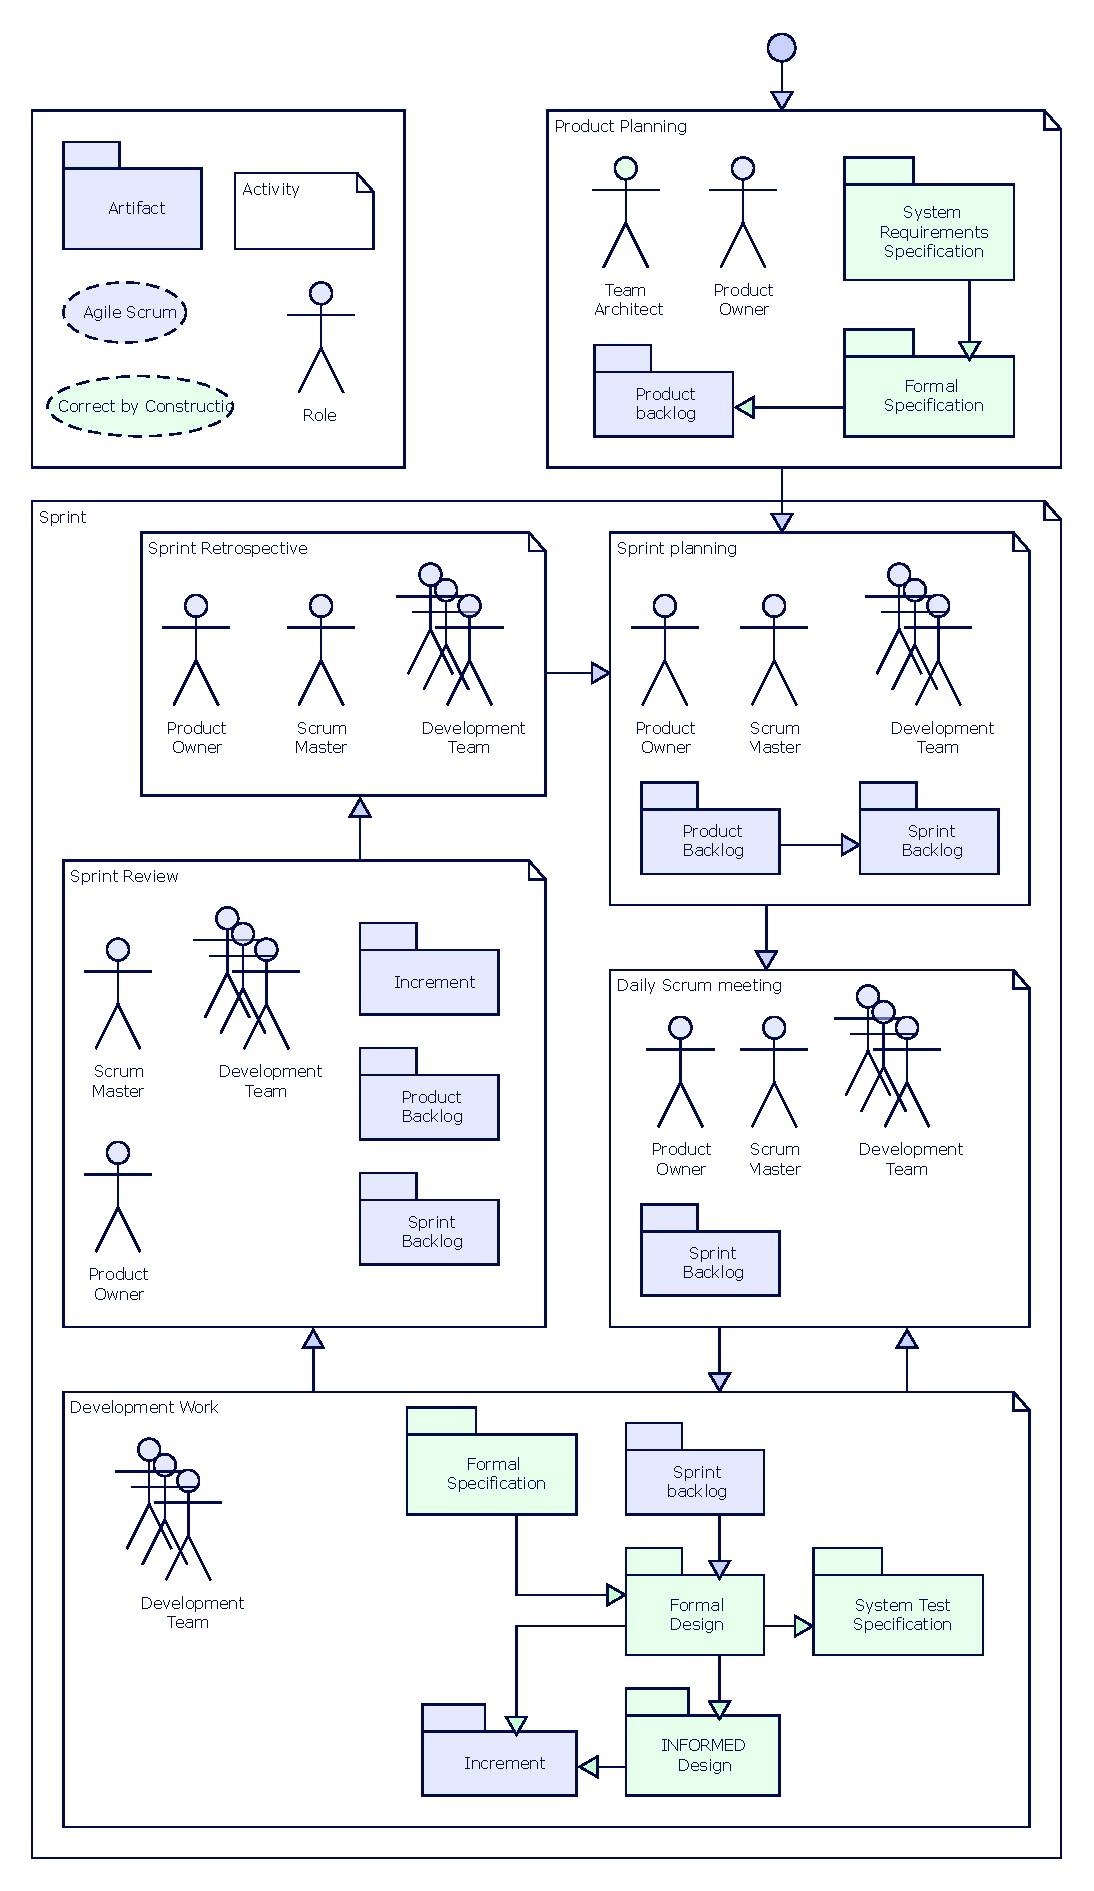
\includegraphics[scale=0.75]{Figures/Scrum_CbyC_workflow.pdf}
	\decoRule
	\caption{The scrum workflow augmented with CbyC.}
	\label{fig:ScrumCbyCWorkflow}
\end{figure}






